\documentclass{beamer}
\usepackage{Stil}
\begin{document}
\title[]{Freifunk-MYK}
\subtitle[Freifunk-MYK]{Vortrag in Gevenich}
\author[Freifunk-MYK]{Norbert Härig, Michael Lambert}
\date{15.03.18\\\vspace{0.5cm} 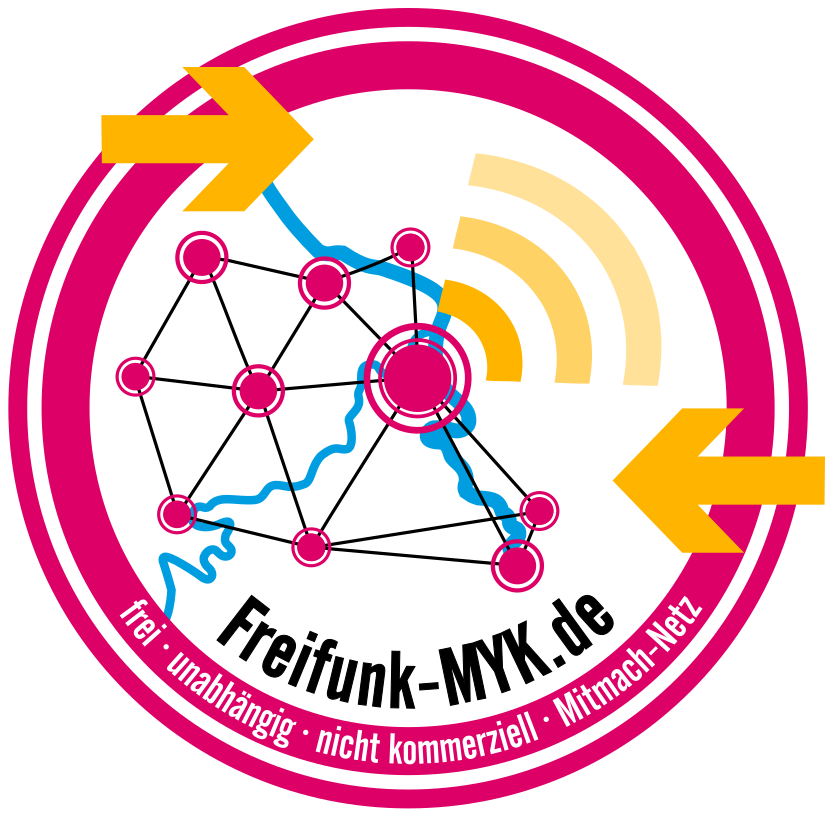
\includegraphics[scale=0.1]{Bilder/Logo.png}}
\institute{}

\begin{frame}
\titlepage	
\end{frame}
% und hier beginnt die Präsentation
\begin{frame}{Referenten}
\begin{itemize}
	\item Norbert Härig
	\begin{itemize}
		\item Brohl
		\item Student
		\item Freifunker seit 2014
	\end{itemize}
	\item Michael Lambert
	\begin{itemize}
		\item Sinzig
		\item EDV-Koordinator Schulen im Kreis Ahrweiler
		\item Freifunker seit 2016
	\end{itemize}
\end{itemize}
\end{frame}

\begin{frame}{Freie Netzwerke - Wozu?}
\begin{itemize}
\item Informations- und Kommunikationsfreiheit im Internet wird zunehmend eingeschränkt
\item „Digital Divide“ - ärmere oder technisch weniger versierte Menschen nehmen wenig oder gar nicht am sogenannten Informationszeitalter teil
\item Internetzugang besonders für Flüchtlinge wertvoll zur Kontaktaufnahme mit der Heimat und als Informationsquelle (Ärzte, Infos über die Stadt, ...)
\item Besser ein Netz, das der Gemeinschaft gehört als eins, das von wenigen Großkonzernen kontrolliert wird
\end{itemize}
\end{frame}

\begin{frame}{\glqq Aber wir haben doch Mobilfunk!\grqq}
WLAN vs. Mobilfunk
\begin{itemize}
\item Geringe Abdeckung in ländlichen Regionen
\item Je nach Tarif teuer und limitiert (besonders für Touristen)
\item Geräte ohne SIM (Notebooks) sind auf WiFi angewiesen
\end{itemize}

\end{frame}



\begin{frame}{Rechtliches zum WLAN freigeben}
\begin{itemize}
\item Seit 2017 Keine Störerhaftung mehr.
\item \glqq Providerprivileg\grqq (TMG § 7(2)  bis § 10)
\item Trotzdem Forderungen von \glqq Abmahn-Anwälten\grqq möglich die abgelehnt werden können
\item Bei Straftaten: Hausdurchsuchungen beim Anschlussinhaber
\end{itemize}
\end{frame}

\begin{frame}{Was ist Freifunk?}
Freifunk ist eine nicht-kommerzielle Initiative, die die Idee freier Netzwerke fördert. \\ 
Frei verstehen wir dabei als:
\begin{itemize}
\item \textbf{öffentlich} (jeder/jedem zugänglich)
\item \textbf{nicht kommerziell} (d.h. keiner Geschäftsstrategie unterworfen)
\item im Besitz einer \textbf{Gemeinschaft} (nicht im Besitz einzelner)
\item \textbf{unzensiert}
\end{itemize}
\end{frame}

\begin{frame}{Vorteile von Freifunk}
\begin{itemize}
\item Keine Vorschaltseite
\item Kein Login/Passwort/Anmeldung erforderlich
\item Ein Netzwerkname (freifunk-myk.de) Geräte wählen sich überall ein 
\item Einfach Skalierbar („Mesh“)
\end{itemize}
\end{frame}

\begin{frame}{Und wie machen wir das?}
\begin{itemize}
\item Freifunkrouter \textbf{erweitern} einen existierenden Anschluss
\item Spezialfirmware auf dem Router leitet Internetverkehr nicht direkt ins \glqq Internet\grqq sondern zu unseren Servern, von da dann ins Internet
\item Nicht Ihre IP steht im „Absender“, sondern unsere
\item Wir leiten weiter zu Freifunk-Rheinland, der die „Anwaltspost“ übernimmt
\end{itemize}
\end{frame}

\begin{frame}{Und wie machen wir das?}
\begin{figure}
\centering
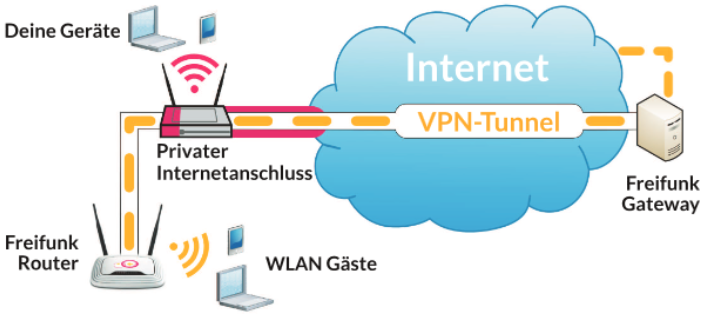
\includegraphics[width=1.0\linewidth]{Bilder/VPN}
\label{fig:vpn}
\end{figure}
\end{frame}

\begin{frame}{Kosten von Freifunk-MYK}
Für den Knotenbetreiber
\begin{itemize}
\item Anschaffung des Routers
\item Internet (Flatrate?)
\item Strom
\end{itemize}
Server
\begin{itemize}
\item ca. 200 Euro pro Monat
\item werden von Freiwilligen betrieben
\item Freifunk-MYK kein Verein $\to$ keine Spendenquittung
\end{itemize}
Uplink zu Freifunk-Rheinland (Anwaltspost)
\begin{itemize}
\item für uns kostenfrei
\item Spendenfinanziert: \url{https://www.freifunk-rheinland.net/spenden}
\end{itemize}

\end{frame}

\begin{frame}{Freifunk in Brohl}
TODO

\end{frame}



\begin{frame}{Jugendraum Brohl 7. Juli 2016}
\begin{figure} 
\centering
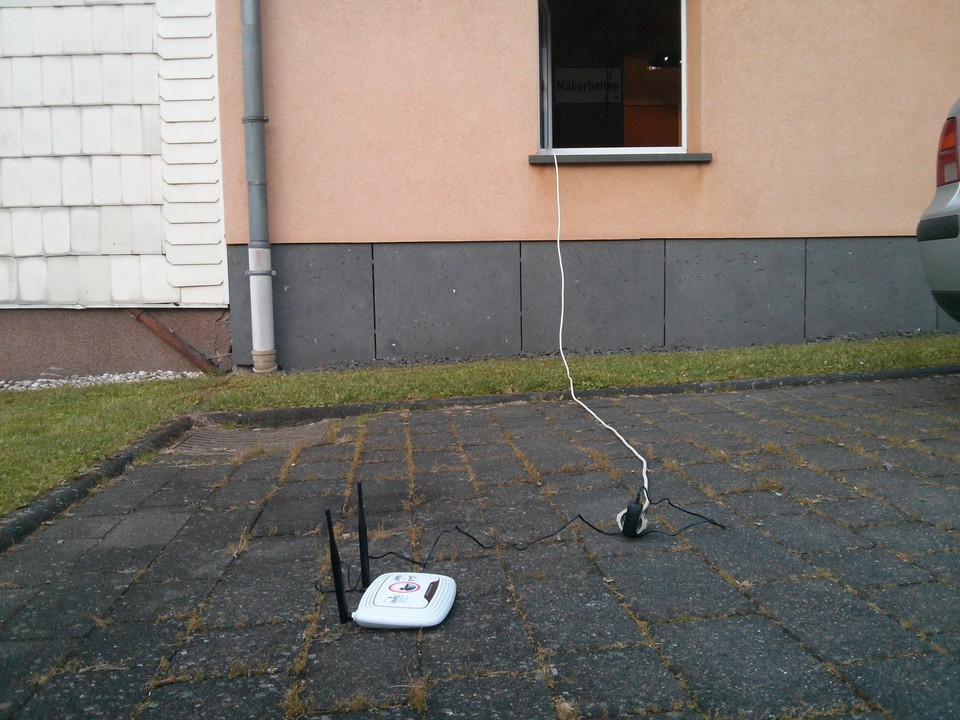
\includegraphics[width=0.8\linewidth]{Bilder/Brohl2016-7-7}
\label{fig:brohl-7}
\end{figure}
\end{frame}



\begin{frame}{Freifunk in Lahr}

\begin{figure}
	\centering
	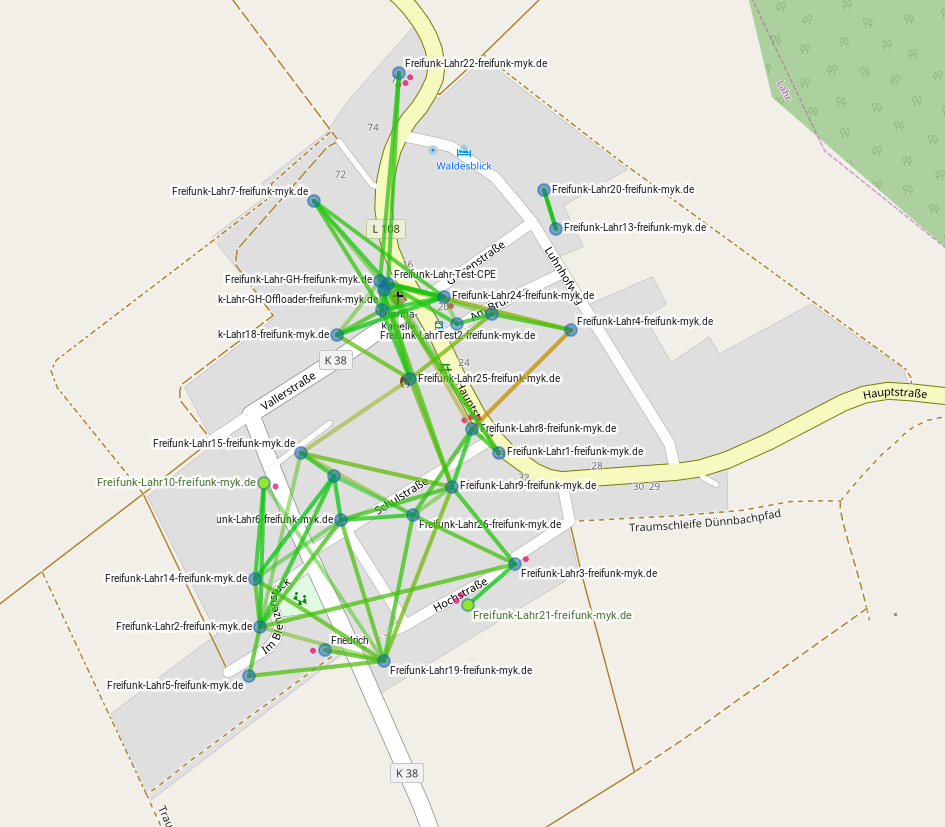
\includegraphics[width=0.7\linewidth]{Bilder/Lahr}
	\caption{}
	\label{fig:lahr}
\end{figure}

\end{frame}

\begin{frame} {Organisation von Freifunk}
\begin{itemize}
\item freifunk.net bundesweit, verbindet lokale Gruppen
Lokale Gruppen, teilweise als e.V
\item In RLP Freifunk: Trier, MYK, Südpfalz, Weyher, Weinstraße, Haßloch, Alzey-Worms, Bingen e.V., ...
\item Ehrenamtliche und freiwillige Tätigkeit
\begin{itemize}
\item Außendarstellen, Werbung, Support
\item Störungen werden schnell beseitigt, allerdings nicht durch bei Freifunk angestellte Techniker
\item freifunk-myk kein Verein mit Vorstand. Offene Baustellen werden durch Ehrenamtliche bearbeitet (oder auch nicht). Ehrensache
\end{itemize}
\end{itemize}
\end{frame}

\begin{frame}{Was Freifunk nicht ist}
\glqq Ein billiger Telekom-Ersatz\grqq - Florian
\begin{figure}
\centering
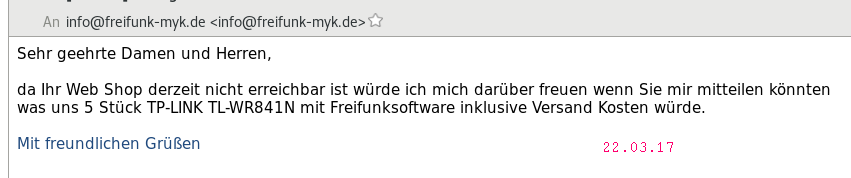
\includegraphics[width=1.0\linewidth]{Bilder/Webshopmail}
\label{fig:webshopmail}
\end{figure}
\end{frame}

\begin{frame} {Zusammenfassung}
\begin{itemize}
\item Dienstbereitstellung erfolgt ausschließlich auf freiwilliger Basis
\item Keinerlei Nutzungsgarantie
\item Entgelte werden nachbarschaftlich geregelt (z.B. für Wartung/Pflege der WLAN-Router, DSL)
\item Kein kommerzielles Angebot
\item Haftung – Aus unserer Sicht gilt: verantwortlich ist immer, wer die unerlaubte Handlung vollführt, nicht wer den Freifunk-Knoten bereitstellt, dagegen spricht die sogenannte Störerhaftung, die wir ablehnen.
\end{itemize}
\end{frame}

\begin{frame} {Quellen/Lizenzierung}
\begin{itemize}
\item Bild mit dem VPN: Freifunk in Landshut und Umgebung Freifunk Altdorf e.V.
\item Folienvorlage von Freifunk Münster
 \url{https://github.com/FreiFunkMuenster/media-ffms/tree/master/Vorlagen/Pr\%C3\%A4sentationen}
\item Dieses Werk ist lizenziert unter CC BY SA 4.0
\end{itemize}
\end{frame}

\end{document}